\documentclass[tikz,border=2pt]{standalone}
\usepackage{amsmath,amssymb}
\usepackage{tikz}

\begin{document}
% A or B (union: either happens) versus A and B (intersection: both happen).
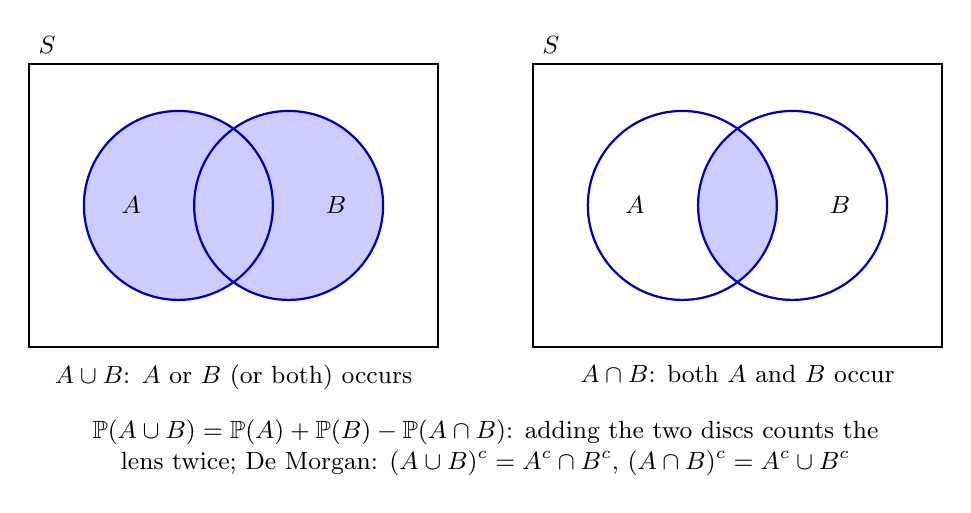
\begin{tikzpicture}[every node/.style={font=\small}]
	\begin{scope}
		\draw[thick] (-2.6,-1.8) rectangle (2.6,1.8);
		\node[anchor=south west] at (-2.6,1.8) {$S$};
		\fill[blue!20] (-0.7,0) circle (1.2);
		\fill[blue!20] (0.7,0) circle (1.2);
		\draw[thick, blue!70!black] (-0.7,0) circle (1.2);
		\draw[thick, blue!70!black] (0.7,0) circle (1.2);
		\node at (-1.3,0) {$A$};
		\node at (1.3,0) {$B$};
		\node[anchor=north] at (0,-1.9) {$A\cup B$: $A$ or $B$ (or both) occurs};
	\end{scope}
	\begin{scope}[xshift=6.4cm]
		\draw[thick] (-2.6,-1.8) rectangle (2.6,1.8);
		\node[anchor=south west] at (-2.6,1.8) {$S$};
		\begin{scope}
			\clip (-0.7,0) circle (1.2);
			\fill[blue!20] (0.7,0) circle (1.2);
		\end{scope}
		\draw[thick, blue!70!black] (-0.7,0) circle (1.2);
		\draw[thick, blue!70!black] (0.7,0) circle (1.2);
		\node at (-1.3,0) {$A$};
		\node at (1.3,0) {$B$};
		\node[anchor=north] at (0,-1.9) {$A\cap B$: both $A$ and $B$ occur};
	\end{scope}
	\node[anchor=north, align=flush center, text width=10cm] at (3.2,-2.6) {$\mathbb{P}(A\cup B)=\mathbb{P}(A)+\mathbb{P}(B)-\mathbb{P}(A\cap B)$: adding the two discs counts the lens twice; De Morgan: $(A\cup B)^c=A^c\cap B^c$, $(A\cap B)^c=A^c\cup B^c$};
\end{tikzpicture}
\end{document}
